\documentclass[conference]{IEEEtran}

\usepackage{amsmath}
\usepackage{amssymb}
\usepackage{graphicx}
\usepackage{float}
\usepackage{booktabs}
\usepackage{tabularx}
\usepackage{tikz}
\usepackage{pgfplots}
\usepackage{cite}
\usepackage{placeins}
\usepackage{algorithm}
\usepackage{algpseudocode}
\usepackage{url}
\usepackage[hidelinks]{hyperref}
\hypersetup{
  pdftitle={Evidence-Driven Dataset Recommendation under Local Resource Constraints},
  pdfauthor={Pratham Kashyap; Anvesha Rastogi; Harsh Gupta; Harsh Dhoriyani; Priyanshu Ranjan; Shrish}
}
\usetikzlibrary{arrows.meta,positioning}
\pgfplotsset{compat=1.18}

\title{Evidence-Driven Dataset Recommendation under Local Resource Constraints}

\author{%
  \begin{tabular}{ccc}
    \parbox[t]{0.31\textwidth}{\centering Pratham Kashyap\\[-1pt]\footnotesize\url{pratham.23bai10455@vitbhopal.ac.in}} &
    \parbox[t]{0.31\textwidth}{\centering Anvesha Rastogi\\[-1pt]\footnotesize\url{anvesha.23bai10355@vitbhopal.ac.in}} &
    \parbox[t]{0.31\textwidth}{\centering Harsh Gupta\\[-1pt]\footnotesize\url{harsh.23bai10402@vitbhopal.ac.in}} \\
    \parbox[t]{0.31\textwidth}{\centering Harsh Dhoriyani\\[-1pt]\footnotesize\url{harsh.23bai10382@vitbhopal.ac.in}} &
    \parbox[t]{0.31\textwidth}{\centering Priyanshu Ranjan\\[-1pt]\footnotesize\url{priyanshu.23bai10691@vitbhopal.ac.in}} &
    \parbox[t]{0.31\textwidth}{\centering Shrish\\[-1pt]\footnotesize\url{shrish.23bai11284@vitbhopal.ac.in}}
  \end{tabular}\\[5pt]
  \IEEEauthorblockA{\textit{School of Computing Science and Artificial Intelligence (SCAI), VIT Bhopal University}\\
  Bhopal-Indore Highway, Kothrikalan, Sehore 466114, Madhya Pradesh, India}
}

\begin{document}
\maketitle

\begin{abstract}
Dataset selection requires more than retrieving descriptions related to a task: compatibility, provenance, bounded content observations, and unresolved claims all affect suitability. We present an implemented local-first pipeline that combines source-attributed evidence states, hard compatibility gates before soft scoring, bounded sample inspection, and traceable set-level selection. On a frozen offline benchmark of 24 datasets and eight structured tasks (192 task--dataset evaluations, target set size $k=3$), mean utility rose from 0.4414 for hybrid reciprocal-rank fusion to 0.8189 after hard gating, then remained at 0.8588 from utility-only ranking through the full system. A separate diversity-weight sweep increased mean diversity from 0.5000 to 0.6111 while mean utility decreased by 0.0089. The M8 path used 33.11 MiB peak memory and 327.49 ms with verified zero network egress. These are bounded observations, not evidence of web-scale effectiveness, independent recommendation quality, or downstream model gains. A three-participant card pilot is descriptive only.
\end{abstract}

\begin{IEEEkeywords}
Dataset recommendation, provenance, evidence representation, task-specific utility, bounded selection.
\end{IEEEkeywords}

\section{Introduction}
Choosing a dataset shapes what a machine-learning task can measure and which populations, conditions, and labels it represents. Dataset search services help users discover candidates across distributed repositories~\cite{noy2019googledatasetsearch}. A textually relevant result, however, does not establish that its modality, target, access conditions, sample contents, or provenance meet a task's requirements. Repository metadata are claims that can be absent or inconsistent, and unrestricted content inspection or dense indexes may exceed a local resource budget.

This paper studies the integration and measured behavior of an evidence-aware recommendation pipeline. It consumes structured task specifications, retains source attribution, separates observation from cross-source resolution, inspects bounded samples, rejects confirmed incompatibilities before ranking, estimates task utility with fixed heuristics, and emits traceable recommendation cards. The M8 evaluation uses a frozen local candidate corpus and records zero network egress; the term \emph{local-first} refers to this execution path, not to a guarantee about every optional component.

\textbf{Research question.} How can a local-first pipeline combine hard task compatibility, source-attributed evidence states, bounded content observations, and set-level selection under an explicit resource envelope, and what measurable behavior does that integration exhibit on fixed development and offline corpora?

The contribution is an evaluated system integration organized around three choices: (1) source-attributed evidence with explicit unknown, failed, unsupported, and conflicting states; (2) hard compatibility constraints before soft ranking; and (3) bounded, traceable recommendation-set selection whose diversity behavior is measured separately from utility. This is not a learned ranking algorithm. The utility components and ranking weights are fixed heuristics, and the set selector carries no formal submodularity or approximation guarantee.

The evidence has different scopes. M2 is a small retrieval component comparison; M3--M7 are development-corpus studies; M8 is a frozen offline benchmark of 24 records and eight tasks. Reference labels were authored for this project before M8 evaluation and without access to its scores. They are not independent ground truth. The paper therefore reports system behavior on these specified corpora rather than general catalog performance.

\section{Related Work}
\subsection{Discovery and task-conditioned recommendation}
Google Dataset Search supports discovery over publisher-provided descriptions~\cite{noy2019googledatasetsearch}. DataFinder studies dataset recommendation from natural-language research descriptions and provides an expert-annotated query set for retrieval evaluation~\cite{viswanathan2023datafinder}. These approaches motivate candidate discovery, while this work treats retrieval rank as one input to suitability assessment rather than as a compatibility decision.

DatasetResearch studies agent-based discovery and synthesis from real-world data demands, reporting a benchmark of 208 demands and a 22\% score for advanced deep-research systems on its challenging \emph{DatasetResearch-pro} subset~\cite{li2025datasetresearch}. Its demand-driven agent setting differs from this paper's fixed-corpus, evidence-ledger pipeline; the results are not a head-to-head comparison.

\subsection{Metadata, provenance, and data quality}
Croissant provides a machine-readable representation for dataset metadata~\cite{akhtar2024croissant}, while Data Cards support human-oriented documentation~\cite{pushkarna2022datacards}. Neither the presence of structured metadata nor documentation makes each value an independently verified observation. The Data Provenance Initiative reports widespread omissions and miscategorization in dataset licensing and attribution records~\cite{longpre2024dataprovenance}. That audit motivates retaining source and uncertainty; it does not establish the correctness or incorrectness of an individual license record in our corpus. License metadata in this system remains a claim, not legal advice.

DataPerf evaluates data-centric methods across tasks such as data selection and debugging~\cite{mazumder2023dataperf}; Confident Learning studies potential label errors using model predictions~\cite{northcutt2021confident}. Our bounded sample diagnostics do not train downstream probes or reproduce those methods. Likewise, GIST provides a formal treatment of max-min diversification with submodular utility~\cite{fahrbach2025gist}; our selector is a simpler deterministic family-aware heuristic and makes no corresponding guarantee.

\section{System and Method}
\subsection{Task, evidence, and bounded inspection}
A structured task specification records task type, modality, domain, target and input needs, scale, governance and access constraints, and unresolved requirements. Free-form language parsing is outside the implemented interface. Canonical dataset records retain source-specific provenance separately from fields exposed to ranking.

Each evidence entry describes a source-attributed claim or observation, including source field, procedure, timestamp, and (when relevant) sample scope. Its observation state is one of \texttt{observed}, \texttt{single\_source\_claim}, \texttt{unsupported}, \texttt{failed}, or \texttt{unknown}. A separate resolution state describes agreement across entries: \texttt{unresolved}, \texttt{corroborated}, \texttt{conflicting}, or \texttt{unknown}. These categorical states are not confidence values. Fingerprinting is bounded to at most 32 records and 64 MiB per dataset; a sample-level observation is not generalized to the full dataset.

The two state layers answer different questions. The observation state describes one evidence entry: a direct sample observation is distinct from a publisher claim, a missing field, an unsupported route, or a failed request. The resolution state describes relationships among entries about the same claim. If two sources disagree, the system preserves that conflict instead of choosing one as truth. This keeps absence of evidence separate from evidence of incompatibility. Source-specific fields remain attached to their adapter provenance and do not become ranking features without canonicalization.

Bounded fingerprints record structural and content summaries only when acquisition is supported by the source policy. A failed endpoint produces a failure state, and an unsupported sampling route remains unsupported; neither becomes a zero-valued observation. Diagnostics such as null-cell rate, duplicate-record rate, column types, or observed target frequencies are interpreted within the sampled rows. They do not estimate full-dataset quality unless a separate sampling design supports that inference, which is outside this study.

Table~\ref{tab:evidence-states} distinguishes the two state layers and the treatment of each state. The observation state is attached to one entry, while resolution summarizes the relation among entries about the same claim. In particular, a failed or unsupported operation does not become an observed absence, and conflicting claims remain visible rather than being averaged or selected by an implicit source preference.

\begin{table*}[!t]
\caption{Evidence state semantics and interpretation}
\label{tab:evidence-states}
\centering
\footnotesize
\begin{tabularx}{\textwidth}{p{0.86in}p{1.48in}X p{2.0in}}
\toprule
Layer & State & Meaning & Interpretation in this study\\
\midrule
Observation & \texttt{observed} & Directly measured or verified through a bounded probe or parse & Evidence is limited to the recorded procedure and sample scope.\\
Observation & \texttt{single\_source\_claim} & Asserted by one publisher or documentation source without independent verification & Preserved as an attributed claim, not upgraded to a fact.\\
Observation & \texttt{unsupported} & The operation or access route is disallowed or unavailable by capability or policy & No favorable or unfavorable content value is inferred.\\
Observation & \texttt{failed} & A supported operation was attempted but failed operationally & Failure remains distinct from a measured zero or negative dataset property.\\
Observation & \texttt{unknown} & The property was unstated, missing, or not observed & Missing information remains unknown.\\
Resolution & \texttt{unresolved} & Evidence is single-source or does not establish agreement or conflict & No cross-source conclusion is asserted.\\
Resolution & \texttt{corroborated} & Independent sources agree, or a claim matches a direct observation & Agreement is recorded without a numeric confidence value.\\
Resolution & \texttt{conflicting} & Two or more observations make incompatible assertions & Both claims and their provenance are retained.\\
Resolution & \texttt{unknown} & No evidence exists, or all entries are unknown or failed & The target claim remains undetermined.\\
\bottomrule
\end{tabularx}
\end{table*}

\subsection{Gating, utility, and set selection}
The engine first applies three hard gates: a confirmed modality mismatch; a dataset license claim matching a task's prohibited-license constraint; or a credential-gated Kaggle asset when anonymous public access is required and gated access is disallowed. A gated candidate is excluded before ranking. The license rule operates on a recorded claim and does not make a legal determination.

Let $\mathcal{D}_q$ be the task-conditioned candidate pool. Define $g_1$, $g_2$, and $g_3$ to equal one when a candidate passes, respectively, the confirmed-modality, prohibited-license-claim, and required-anonymous-access gates described above. A modality passes when the task's known required modality is compatible with the recorded modalities (including multimodal or unknown metadata); a license gate applies only when the recorded claim matches a prohibited term; and the access gate applies to Kaggle when public access is required and gated access is disallowed. Eligibility is therefore:
\begin{equation}
\mathcal{D}_q^{\mathrm{eligible}} =
\{d\in\mathcal{D}_q: g_1(q,d)=g_2(q,d)=g_3(q,d)=1\}.
\label{eq:eligibility}
\end{equation}

For eligible candidates, let $u_1,\ldots,u_7$ denote the normalized task, modality, target, structure, quality, governance, and access-feasibility component scores. Task utility is their equal-weight mean:
\begin{equation}
U(q,d)=\frac{1}{7}\sum_{j=1}^{7}u_j(q,d).
\label{eq:utility}
\end{equation}
Equation~\ref{eq:utility} formalizes the equal contribution of those seven component scores for each eligible task--candidate pair.
The five-dimension candidate score---fit, utility, evidence support, content coverage, and risk penalty---uses fixed weights:
\begin{equation}
\begin{aligned}
 s(q,d) &= 0.35F(q,d)+0.35U(q,d)+0.15E(q,d)\\
         &\quad +0.15C(q,d)-0.15R(q,d).
\end{aligned}
\label{eq:score}
\end{equation}
Equations~\ref{eq:eligibility}--\ref{eq:score} separate feasibility from preference: an ineligible candidate is removed before the score orders the eligible pool. These scores are heuristic estimates, not calibrated probabilities. Popularity can appear as context or inform a role, but it is not a direct suitability bonus.

The two score levels should not be conflated. The seven utility components express compatibility estimates used by the task-utility estimator; the five dimensions in Equation~\ref{eq:score} combine that estimate with fit and evidence-related terms for ordering eligible candidates. Fit summarizes task, modality, and target alignment. Evidence support reflects the state and provenance of relevant claims. Content coverage reflects what bounded inspection observed. Risk captures unresolved task-relevant concerns. Weights are specified in the implementation and were not fit on M8 labels.

For the set selector, pairwise attribute distance is the mean of lineage distance, schema-feature distance, and source distance:
\begin{equation}
\operatorname{dist}(a,b)=
\frac{d_{\mathrm{lin}}(a,b)+d_{\mathrm{schema}}(a,b)+d_{\mathrm{src}}(a,b)}{3}.
\label{eq:distance}
\end{equation}
Equation~\ref{eq:distance} is the pairwise distance used both by greedy selection and by the reported diversity statistic.
The lineage term is 0 for a confirmed same family, 1 for a different family, and 0.5 when unresolved. The schema term is Jaccard distance for two nonempty feature-token sets, 0.5 when both are empty, and 0.8 when only one is empty. The source term is 0 for a shared known source and 1 otherwise. The implementation rounds each pairwise distance to four decimal places. Set diversity is the mean of these pairwise distances, rounded to four decimals, with value zero for sets of size at most one:
\begin{equation}
D(S)=
\begin{cases}
0, & |S|\leq 1,\\[2pt]
\displaystyle\frac{2}{|S|(|S|-1)}
\sum_{\{a,b\}\in\binom{S}{2}}\operatorname{dist}(a,b), & |S|>1.
\end{cases}
\label{eq:set-diversity}
\end{equation}
Equation~\ref{eq:set-diversity} computes the mean over unordered pairs and returns zero when fewer than two items are selected.

The selector greedily builds a set up to $k=3$. At each step it excludes candidates that the implemented family-linkage check identifies as a same-family duplicate of any selected item. The marginal diversity contribution is one for the first selection and otherwise the minimum distance to the selected set:
\begin{equation}
\delta(d\mid S)=
\begin{cases}
1, & S=\varnothing,\\
\min_{x\in S}\operatorname{dist}(d,x), & S\neq\varnothing.
\end{cases}
\label{eq:marginal-diversity}
\end{equation}
Equation~\ref{eq:marginal-diversity} matches the selector's explicit empty-set value and its minimum-distance contribution thereafter. Let $\mathcal{A}_q(S_t)$ contain eligible candidates not yet selected that the implemented family-linkage check does not identify as same-family duplicates of items in $S_t$. For $S_0=\varnothing$, each next item is selected as
\begin{equation}
\begin{aligned}
d_t&=\arg\max_{d\in\mathcal{A}_q(S_t)}
\left[s(q,d)+\lambda_{\mathrm{div}}\delta(d\mid S_t)\right],\\
S_{t+1}&=S_t\cup\{d_t\}.
\end{aligned}
\label{eq:selection}
\end{equation}
Equation~\ref{eq:selection} is the implemented bounded greedy step. Selection stops at $k=3$ or when no eligible nonredundant candidate remains; ties use the marginal gain rounded to six decimals, intrinsic score rounded to six decimals, then the lexicographically greatest dataset identifier. The default is $\lambda_{\mathrm{div}}=0.20$. This bounded greedy rule is a heuristic; no formal submodularity claim is made. The resulting cards link selected records to scores, evidence identifiers, fingerprints, and reasons for fit and caveats.

Selection is applied only after gating. Family-aware exclusion uses the implemented corroborated family-linkage decision; the diversity term can still alter composition when no same-family pairs exist because it also considers schema and source attributes. Utility and diversity are reported separately to expose this trade-off. Each result remains specific to the benchmark, its attributes, and the chosen weight.

For a nonempty selected set $S_q$, task-level utility is the mean of its selected candidates' utility values; the eight-task M8 aggregate averages those task means. The implementation assigns zero to an empty set:
\begin{equation}
U(S_q)=
\begin{cases}
\displaystyle\frac{1}{|S_q|}\sum_{d\in S_q}U(q,d), & |S_q|>0,\\
0, & |S_q|=0,
\end{cases}
\label{eq:set-utility}
\end{equation}
and the M8 macro-average across tasks is
\begin{equation}
\bar U=\frac{1}{|Q|}\sum_{q\in Q}U(S_q),
\label{eq:aggregation}
\end{equation}
where $Q$ is the set of eight fixed M8 tasks. In the recorded M8 results all eight selected sets are nonempty. Equations~\ref{eq:set-utility} and~\ref{eq:aggregation} match the recorded per-task set utility and subsequent arithmetic mean; tasks are not weighted by set size.

Recommendation cards expose dataset and task identifiers, rank, component signals, utility estimate, evidence-entry and fingerprint references, selection role, and structured reasons for fit and caveats. The associated set record retains selected identifiers, aggregate utility and diversity, gate exclusions, target size, and diversification parameter. This gives a trace from the displayed recommendation to recorded evidence without presenting a claim as independently verified.

The design envelope derived in M0 is a 128 MiB process ceiling, a 20,000 ms cold per-task budget, and the bounded sample limit above. These are project design limits, not a guarantee that every optional backend meets them.

The implemented flow keeps candidate discovery, evidence processing, and selection as traceable stages (Fig.~\ref{fig:pipeline}). Source adapters preserve native provenance in canonical records. The evidence ledger stores claims and observations, while fingerprints retain bounded sample scope. Gating precedes utility and multi-objective scoring. The selector then constructs the set and emits cards linked to the evidence used. M8 starts from its frozen corpus and does not invoke the retrieval stage as a live search operation.

Algorithm~\ref{alg:pipeline} summarizes the implemented decision order. Its inputs include the candidate records and their recorded evidence and fingerprints; live retrieval is outside the M8 evaluation. The stopping rule is bounded by the target set size or exhaustion of candidates that pass the gates and family check.

\begin{algorithm}[t]
\caption{Evidence-linked recommendation from a supplied candidate pool}
\label{alg:pipeline}
\footnotesize
\begin{algorithmic}[1]
\Require task $q$, candidate pool $\mathcal{D}_q$, evidence ledger $E$, fingerprints $F$, $k=3$, $\lambda_{\mathrm{div}}$
\Ensure selected cards with linked evidence and caveats
\State $S\gets\emptyset$; $\mathcal{D}_q^{\mathrm{eligible}}\gets\emptyset$
\ForAll{$d\in\mathcal{D}_q$}
  \State retain source-attributed entries $E_d$ and bounded observations $F_d$
  \State compute the seven-component task utility and evaluate the three hard gates
  \If{$d$ passes all gates}
    \State compute fixed five-dimension score $s(q,d)$; add $d$ to $\mathcal{D}_q^{\mathrm{eligible}}$
  \EndIf
\EndFor
\While{$|S|<k$}
  \State $A\gets$ eligible, unselected candidates not linked as same-family to any item in $S$
  \If{$A=\emptyset$} \State \textbf{break} \EndIf
  \State choose $d\in A$ maximizing $s(q,d)+\lambda_{\mathrm{div}}\delta(d\mid S)$ with implemented tie-breaks
  \State $S\gets S\cup\{d\}$
\EndWhile
\State emit cards for $S$ with score, evidence identifiers, fingerprint scope, and recorded reasons
\end{algorithmic}
\end{algorithm}

\begin{figure*}[t]
\centering
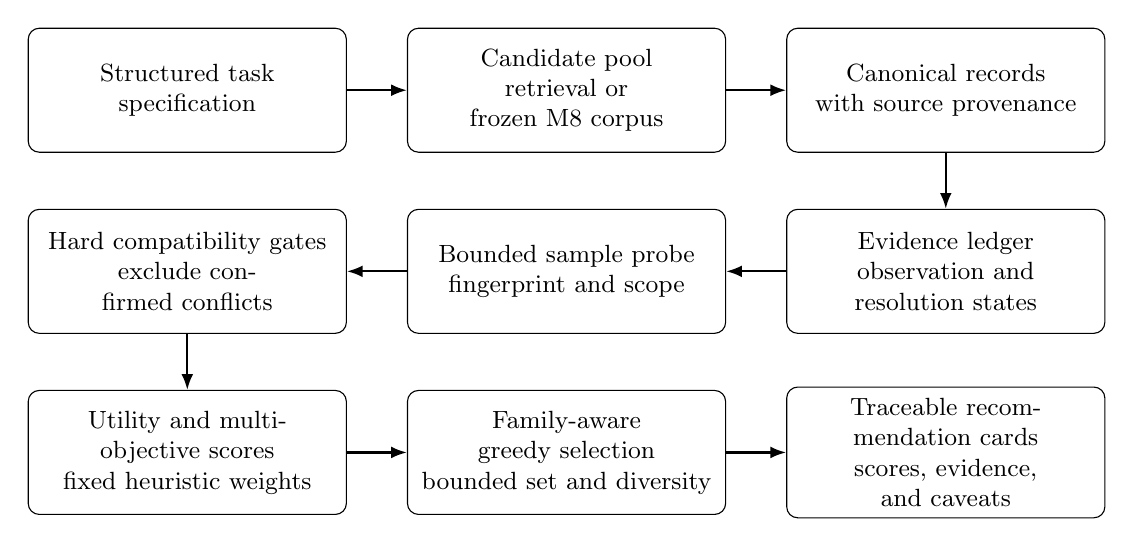
\begin{tikzpicture}[
  node distance=0.28in and 0.30in,
  box/.style={draw,rounded corners,align=center,text width=1.48in,minimum height=0.62in,inner sep=4pt,font=\small},
  arrow/.style={-{Latex[length=2mm]},thick}
]
\node[box] (task) {Structured task specification};
\node[box,right=of task] (pool) {Candidate pool\\retrieval or frozen M8 corpus};
\node[box,right=of pool] (canon) {Canonical records\\with source provenance};
\node[box,below=of canon] (evidence) {Evidence ledger\\observation and resolution states};
\node[box,left=of evidence] (sample) {Bounded sample probe\\fingerprint and scope};
\node[box,left=of sample] (gate) {Hard compatibility gates\\exclude confirmed conflicts};
\node[box,below=of gate] (rank) {Utility and multi-objective scores\\fixed heuristic weights};
\node[box,right=of rank] (select) {Family-aware greedy selection\\bounded set and diversity};
\node[box,right=of select] (cards) {Traceable recommendation cards\\scores, evidence, and caveats};
\draw[arrow] (task) -- (pool);
\draw[arrow] (pool) -- (canon);
\draw[arrow] (canon) -- (evidence);
\draw[arrow] (evidence) -- (sample);
\draw[arrow] (sample) -- (gate);
\draw[arrow] (gate) -- (rank);
\draw[arrow] (rank) -- (select);
\draw[arrow] (select) -- (cards);
\end{tikzpicture}
\caption{Implemented recommendation flow. The M8 evaluation supplies the frozen candidate pool directly; retrieval is evaluated separately and is not measured as live M8 recall.}
\label{fig:pipeline}
\end{figure*}

\subsection{Evaluation settings and interpretation}
M2 compares BM25, MiniLM dense retrieval, and reciprocal-rank fusion (RRF) on ten development records, four manually curated queries, and five relevance pairs derived from source descriptions. The benchmark reports Recall@1/3, latency, model/index preparation time, and process memory. Each method/query timing is a single measured call without a warm-up call or repeats; results are descriptive.

The lexical and dense rank lists are fused with reciprocal-rank fusion using the recorded configuration. M2 relevance labels were formed from source descriptions for a small component comparison, not from an independent relevance panel. The shared process-level peak RSS cannot support an isolated memory comparison for BM25.

M3--M7 use a ten-record development corpus. M3 records evidence claims; M4 fingerprints accessible bounded samples; M5 compares metadata-only, evidence-ledger, and fingerprint-augmented utility baselines against a project-authored rubric; M6 is a standalone exploratory pool simulation; M7 compares utility-only (R1), multi-objective (R2), and family-aware greedy (R3) selection. M6 does not feed M8.

M5's three configurations add information in stages: A uses metadata only, B adds the M3 evidence ledger, and C also uses M4 fingerprints. Each is compared with the same project-authored rubric over four task specifications and ten records. This is a within-project ranking-consistency check. Shared task-compatibility concepts between rubric and estimator mean that agreement is not an external measure of predictive usefulness or downstream model performance.

M8 evaluates 24 frozen records against eight structured tasks (192 task--dataset pairs), with target $k=3$, seed 20260902, and the candidate corpus passed directly to the engine. One Kaggle Heart Disease record was excluded after an HTTP 403 response under the recorded access policy. The ablation's retrieval conditions reorder or rank this same pool. They are not live retrieval runs and do not measure end-to-end retrieval recall. The recorded run was on macOS arm64/Python 3.14.6, with network egress forbidden and zero egress verified. The reference labels were recorded before the M8 harness ran and without seeing M8 scores; the same project author produced them, with no independent annotator, inter-annotator agreement, or external validation.

For each task, the supplied pool contains the same 24 records in the frozen manifest order; the estimator and gates determine which are eligible for ranking. This protocol deliberately conditions all ranking comparisons on that common pool, so changes across ablation rungs can be associated with the configured ordering, eligibility, scoring, or selection stage within this harness. It cannot answer whether a live retriever would find a relevant dataset missing from the pool. The evaluation also uses one fixed task specification per task family and a target set size of three; results do not measure sensitivity to alternate task wording, user constraints, or recommendation-set sizes.

The M8 conditions are cumulative: corpus order; BM25 ordering; dense ordering; hybrid RRF ordering; hybrid ordering plus hard gates; utility-only ranking (R1); multi-objective ranking (R2); farthest-first selection without a family check; and the full system (R3). Mean set utility is calculated per task as the arithmetic mean utility of selected items, then averaged equally across the eight tasks. Since four tasks have two selected items after gating while the other four retain three, rung-to-rung changes are influenced by eligibility and set size. R0 is a corpus-order reference condition, not a generally failing algorithm.

The registered M8 hypotheses distinguish descriptive behaviors from architecture checks. H1 tests same-family redundancy elimination only when an R1 top-$k$ set contains an eligible pair; H2 measures reordering among utility-near divergent pairs; H3 tests utility retention at tolerance $\epsilon=0.03$; H4 separates exclusion of popularity from direct scoring from an empirical task-level association test; and H5 checks that recommendation roles have grounding evidence. Table~\ref{tab:protocol} summarizes the evaluation scopes and their boundaries. None of these outcomes is a general performance guarantee.

\begin{table*}[t]
\caption{Evaluation settings and protocol boundaries}
\label{tab:protocol}
\centering
\footnotesize
\begin{tabularx}{\textwidth}{p{1.1in}p{1.35in}X p{1.6in}}
\toprule
Setting & Corpus and task scope & Protocol & Interpretation boundary\\
\midrule
M0 envelope & Local process measurements & Cold-request and sample-access measurements informed design ceilings & 128 MiB process ceiling; 20,000 ms cold per-task budget; 32 records / 64 MiB per sample\\
M2--M7 development & 10 canonical records; four queries or tasks as specified & Component retrieval, ledger, sample fingerprint, rubric, exploration, and ranking studies & M5 rubric labels are project-authored; studies are not a sample of the full catalog\\
M8 frozen benchmark & 24 records $\times$ 8 tasks = 192 pairs; $k=3$ & Fixed corpus, deterministic run, seed 20260902; robustness and sensitivity fixtures separate & macOS arm64/Python 3.14.6; zero egress verified; no web-scale or downstream-model evaluation\\
\bottomrule
\end{tabularx}
\end{table*}

\section{Results}
\subsection{M8 hard-gating jump and post-gating plateau}
The principal M8 result is the rise in mean set utility from 0.4414 at hybrid RRF to 0.8189 after hard gating. Utility-only ranking then reached 0.8588, and multi-objective scoring, farthest-first selection without family checks, and the full system each remained at 0.8588. Table~\ref{tab:ablation} reports the cumulative ladder. Thus hard gating accounts for the largest observed change in this cumulative ablation, while the later stages form a flat mean-utility plateau on this corpus and rubric.

\begin{table}[t]
\caption{M8 cumulative ablation over the fixed candidate pool}
\label{tab:ablation}
\centering
\footnotesize
\begin{tabular}{clc}
\toprule
Rung & Condition & Mean set utility\\
\midrule
0 & Corpus-order reference & 0.2191\\
1 & BM25 only & 0.4684\\
2 & Dense only & 0.4085\\
3 & Hybrid RRF & 0.4414\\
4 & Hybrid plus hard gates & 0.8189\\
5 & Utility only (R1) & 0.8588\\
6 & Multi-objective (R2) & 0.8588\\
7 & Farthest-first, no family check & 0.8588\\
8 & Full system (R3) & 0.8588\\
\bottomrule
\end{tabular}
\end{table}

These are cumulative conditions, not isolated causal effects. Rungs 0--3 selected three items per task; after gating, four tasks returned two and four returned three. The 0.4414-to-0.8189 change therefore reflects eligibility and realized set size as well as ranking. The fixed-pool design also means the first four conditions say nothing about live search recall.

\subsection{Diversity--utility sensitivity}
The full eight-point $\lambda_{\mathrm{div}}$ sweep shows that utility alone hides changes in the selected sets. Mean diversity rose from 0.5000 at weights 0.00--0.10 to 0.5278 at 0.15--0.20, 0.5556 at 0.25, and 0.6111 at 0.30--0.40. Mean utility stayed at 0.858825 through 0.20, then fell to 0.855850 at 0.25 and 0.849950 at 0.30--0.40. Diversity increased by 0.1111 at the high settings while utility decreased by 0.008875 (about 0.0089). Membership changed despite zero qualifying same-family pairs in M8.

Figure~\ref{fig:lambda-sweep} shows the plateau and trade-off across the recorded settings; Table~\ref{tab:lambda} retains the exact values and set-overlap measure.

\begin{figure}[t]
\centering
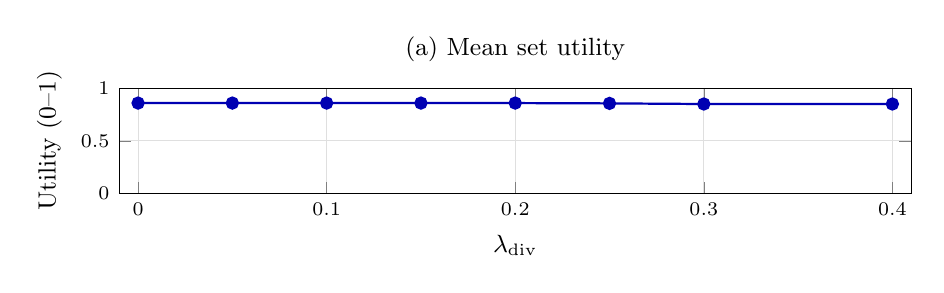
\begin{tikzpicture}
\begin{axis}[
  width=0.96\columnwidth,height=1.15in,
  title={(a) Mean set utility},
  xlabel={$\lambda_{\mathrm{div}}$},ylabel={Utility (0--1)},
  xmin=-0.01,xmax=0.41,ymin=0,ymax=1,
  xtick={0,0.10,0.20,0.30,0.40},
  ytick={0,0.5,1.0},
  xticklabel style={font=\scriptsize},
  yticklabel style={font=\scriptsize},
  label style={font=\small},title style={font=\small},
  grid=major,grid style={gray!25}
]
\addplot[blue!70!black,mark=*,thick] coordinates {
  (0.00,0.858825) (0.05,0.858825) (0.10,0.858825) (0.15,0.858825)
  (0.20,0.858825) (0.25,0.855850) (0.30,0.849950) (0.40,0.849950)
};
\end{axis}
\end{tikzpicture}
\\[-2pt]
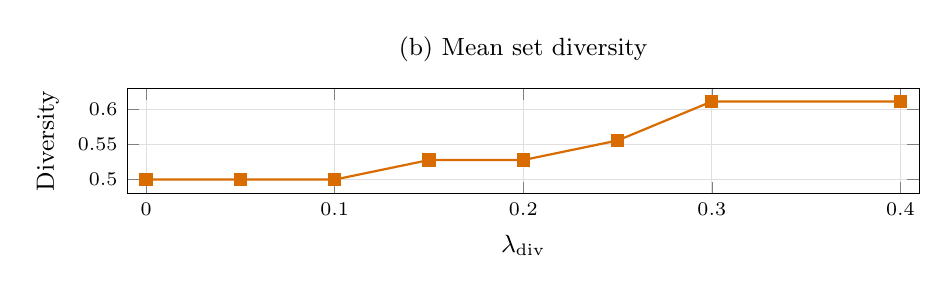
\begin{tikzpicture}
\begin{axis}[
  width=0.96\columnwidth,height=1.15in,
  title={(b) Mean set diversity},
  xlabel={$\lambda_{\mathrm{div}}$},ylabel={Diversity},
  xmin=-0.01,xmax=0.41,ymin=0.48,ymax=0.63,
  xtick={0,0.10,0.20,0.30,0.40},
  xticklabel style={font=\scriptsize},
  yticklabel style={font=\scriptsize},
  label style={font=\small},title style={font=\small},
  grid=major,grid style={gray!25}
]
\addplot[orange!85!black,mark=square*,thick] coordinates {
  (0.00,0.5000) (0.05,0.5000) (0.10,0.5000) (0.15,0.527775)
  (0.20,0.527775) (0.25,0.55555) (0.30,0.6111) (0.40,0.6111)
};
\end{axis}
\end{tikzpicture}
\caption{M8 diversity-weight sensitivity over eight fixed tasks: (a) mean set utility on its full normalized 0--1 scale and (b) mean set diversity. Utility is unchanged through $\lambda_{\mathrm{div}}=0.20$, then declines as diversity increases at higher settings. The full-scale utility axis avoids visually magnifying the small change; Table~\ref{tab:lambda} reports the exact values and mean Jaccard against the default.}
\label{fig:lambda-sweep}
\end{figure}

\begin{table}[t]
\caption{M8 $\lambda_{\mathrm{div}}$ sensitivity (means over eight tasks)}
\label{tab:lambda}
\centering
\footnotesize
\begin{tabular}{cccc}
\toprule
$\lambda_{\mathrm{div}}$ & Mean utility & Mean diversity & Jaccard vs. 0.20\\
\midrule
0.00 & 0.858825 & 0.5000 & 0.9375\\
0.05 & 0.858825 & 0.5000 & 0.9375\\
0.10 & 0.858825 & 0.5000 & 0.9375\\
0.15 & 0.858825 & 0.5278 & 1.0000\\
0.20 & 0.858825 & 0.5278 & 1.0000\\
0.25 & 0.855850 & 0.5556 & 0.9375\\
0.30 & 0.849950 & 0.6111 & 0.8125\\
0.40 & 0.849950 & 0.6111 & 0.8125\\
\bottomrule
\end{tabular}
\end{table}

The sweep is finite and does not establish stability outside these values. The $\epsilon=0.03$ threshold belongs to the registered utility-retention hypothesis, not to a separate sensitivity criterion. In M8, H1 was not applicable because no R1 top-$k$ set contained a qualifying same-family pair. This does not negate the separate M7 development observation.

The task-level records qualify the aggregate plateau. Across $\lambda_{\mathrm{div}}=0.00$ through $0.20$, macro mean utility remains 0.858825, even though the tabular-diabetes selected set differs at 0.00--0.10 and returns to the default membership by 0.15. At 0.25, the Iris set changes and macro utility is 0.855850; at 0.30 and 0.40, Iris, Titanic, and wine memberships differ from the default, and macro utility is 0.849950. At $\lambda_{\mathrm{div}}=0.40$, utility falls from 0.8809 to 0.8571 for Iris, from 0.9283 to 0.9045 for Titanic, and from 0.8568 to 0.8334 for wine; the other five task-level utilities remain unchanged. These three decreases limit the macro-average decline from 0.20 to 0.40 to 0.008875. Thus, the diversity increase is not utility-free for every affected task, and the aggregate result should not be interpreted as ranking or membership invariance. The observed plateau is specific to these tasks, candidates, and eight tested weights.

This heterogeneity is concentrated in the tabular tasks. Across the full sweep, the two image tasks and two text tasks retain the same selected membership, utility, and diversity. Diabetes has a membership change at the three lowest tested weights but retains mean set utility 0.9045; its diversity is 0.7222 from the default weight onward. Iris, Titanic, and wine retain their default sets through $\lambda_{\mathrm{div}}=0.20$, then reach Jaccard 0.5 against the default at 0.25 or above. At 0.40, their task utilities are 0.8571, 0.9045, and 0.8334, respectively, and each has set diversity 0.7222. These task records show that the aggregate utility cost is localized to three of eight tasks in the tested endpoint comparison. They do not identify a universally preferred weight or support extrapolation beyond this frozen pool.

Table~\ref{tab:task-sensitivity} makes this concentration visible without collapsing tasks into a single macro-average. At the default weight, set utility varies from 0.7786 on both image tasks to 0.9283 on Titanic; at 0.40, only Iris, Titanic, and wine change utility, while the other five task-level values remain constant. Jaccard is computed against each task's selected set at the default $\lambda_{\mathrm{div}}=0.20$; a value of 0.5 indicates partial membership overlap, not a rank-correlation measure.

\begin{table*}[!t]
\caption{M8 task-level sensitivity endpoints at $\lambda_{\mathrm{div}}=0.20$ and $0.40$}
\label{tab:task-sensitivity}
\centering
\footnotesize
\begin{tabular}{lccccc}
\toprule
Task & $U_q$ at 0.20 & $D_q$ at 0.20 & $U_q$ at 0.40 & $D_q$ at 0.40 & Jaccard at 0.40\\
\midrule
Image--CIFAR & 0.7786 & 0.5000 & 0.7786 & 0.5000 & 1.0\\
Image--leaf disease & 0.7786 & 0.5000 & 0.7786 & 0.5000 & 1.0\\
News--multiclass & 0.8500 & 0.5000 & 0.8500 & 0.5000 & 1.0\\
Sentiment--binary & 0.8929 & 0.5000 & 0.8929 & 0.5000 & 1.0\\
Tabular--diabetes & 0.9045 & 0.7222 & 0.9045 & 0.7222 & 1.0\\
Tabular--Iris & 0.8809 & 0.5000 & 0.8571 & 0.7222 & 0.5\\
Tabular--Titanic & 0.9283 & 0.5000 & 0.9045 & 0.7222 & 0.5\\
Tabular--wine & 0.8568 & 0.5000 & 0.8334 & 0.7222 & 0.5\\
\bottomrule
\end{tabular}
\end{table*}

\subsection{Retrieval and resource trade-off}
On the small M2 development benchmark, BM25, dense MiniLM, and hybrid RRF each reached Recall@1 of 0.875 and Recall@3 of 1.000. The recorded means were 0.0602 ms for BM25, 700.1929 ms for dense retrieval, and 15.0808 ms for hybrid. Dense per-query latency ranged from 16.30 to 1,870.23 ms. Index construction took 81,000.40 ms and embedding generation 5,038.56 ms. The combined retrieval benchmark process reached 475,234,304 bytes (453.22 MiB) peak RSS; memory was not isolated per backend, and BM25 peak RSS was not separately recorded. This one-pass, no-warm-up, no-repeat comparison on four queries does not establish general retrieval superiority. BM25 is the constrained retrieval default; optional dense MiniLM is outside the 128 MiB ceiling.


Table~\ref{tab:m2} summarizes this component comparison.

\begin{table}[t]
\caption{M2 retrieval comparison}
\label{tab:m2}
\centering
\footnotesize
\begin{tabular}{lcccc}
\toprule
Method & R@1 & R@3 & Mean ms/query & Peak RSS\\
\midrule
BM25 & 0.875 & 1.000 & 0.0602 & N/A\\
Dense MiniLM & 0.875 & 1.000 & 700.1929 & Shared process\\
Hybrid RRF & 0.875 & 1.000 & 15.0808 & Shared process\\
\bottomrule
\end{tabular}
\end{table}

The dense MiniLM query-time range was 16.30--1,870.23 ms. The shared process RSS for the benchmark was 453.22 MiB; assigning that value to BM25 alone would be unsupported. The configured dense index-build and embedding-generation phases took 81.0 s and 5.04 s respectively. The measurements are single pass on a recorded macOS arm64/Python 3.14.6 environment. A warmed, repeated and per-backend-isolated benchmark would be needed to support more stable latency or memory comparisons.

By contrast, the frozen M8 offline recommendation path used 33.11 MiB peak RSS and 327.49 ms wall time, with zero egress verified, within the measured M0 ceiling. These figures apply to different execution paths and should not be combined into a claim that every component fits the envelope.

\subsection{M8 registered outcomes}
M8's registered outcomes are summarized in Table~\ref{tab:hypotheses}. H2 reordered 3 of 33 utility-near divergent pairs (9.1\%); H3 met the utility-retention criterion with R1 and R3 both at 0.8588, but no mirror case exercised the family rule; H4's popularity exclusion is an implementation invariant while empirical association was not applicable for all eight tasks; H5 found 20/20 assigned roles met grounding preconditions.

\begin{table}[t]
\caption{M8 registered hypothesis outcomes}
\label{tab:hypotheses}
\centering
\footnotesize
\begin{tabularx}{\columnwidth}{p{0.28in}p{0.75in}X}
\toprule
ID & Status & Observed result and boundary\\
\midrule
H1 & N/A & No R1 top-$k$ set contained a qualifying same-family pair.\\
H2 & Exploratory & 3/33 utility-near divergent pairs reordered (9.1\%); qualifying pairs were drawn from 6/8 tasks; descriptive only.\\
H3 & Criterion met & R1 and R3 utility both 0.8588; retention under this corpus geometry.\\
H4 & Invariant met & Popularity excluded from scoring; association N/A in all eight tasks.\\
H5 & Supported & 20/20 assigned roles met grounding preconditions.\\
\bottomrule
\end{tabularx}
\end{table}

\subsection{Robustness and Internal Consistency}
Four robustness suites covered ten severity trials with zero crashes; Table~\ref{tab:robustness} reports each tested perturbation and its boundary. These fixture outcomes characterize only the tested perturbations. Internal consistency diagnostics over 192 project-authored labels (18 positive) were Brier 0.259314 and five-bin ECE 0.428503; these are not independent calibration estimates.

\begin{table}[t]
\caption{M8 robustness fixtures and internal consistency audit}
\label{tab:robustness}
\centering
\footnotesize
\begin{tabularx}{\columnwidth}{p{0.92in}X}
\toprule
Fixture & Recorded outcome and boundary\\
\midrule
Metadata omission & 3 severities; zero evidence-state transitions and zero crashes. Fixture corruption only.\\
License conflict & 2 severities; 16 state transitions at each severity and zero crashes. Injected conflict; no legal resolution.\\
Modality corruption & 2 severities; hard-gating recall 0.6667, set Jaccard 0.9375, zero crashes. Fixture-specific gating.\\
Endpoint failure & 3 severities; 16/40/40 transitions, mean utility change $-0.00415$ to $-0.00475$, Jaccard 0.9375. Simulated failures.\\
Consistency audit & 192 pairs, 18 positive; Brier 0.259314 and five-bin ECE 0.428503. Related project labels, not calibration.\\
\bottomrule
\end{tabularx}
\end{table}
\subsection{Development-Corpus Results (M3--M7)}
The supporting development results are summarized in Table~\ref{tab:development}. The M3 license conflict records differing source claims; it is not resolved by the Data Provenance Initiative's broad audit. M4's zero null and duplicate rates apply only to evaluated samples, including a 32-row Rotten Tomatoes slice whose observed label was constant. Unsupported access and the Beans HTTP 502 failure remain explicit rather than being treated as favorable observations.

M5's baseline C improved mean Spearman correlation from 0.9576 (A and B) to 0.9667, while NDCG@3/@5/@10 remained 0.5421/0.6094/0.6766 in each configuration. Hard gates excluded 90 of 120 task--candidate evaluations (75\%) in that development comparison. M6 added two under-observed high-utility candidates only for the tabular-wine query, raising that pool's mean utility from 0.5476 to 0.6857; the other three queries had no additions and no candidate met the strict hidden-gem rule.

M3 recorded 107 evidence entries across ten development records. Sixty-seven entries (62.6\%) were single-source claims; among 106 claim resolutions, 90 were unresolved, 15 were unknown, and one was conflicting. The conflict involved a Rotten Tomatoes license string of \texttt{MIT} and a Croissant license URI. The evidence model retains both claims rather than normalizing them into agreement. These counts describe the harvested records, not metadata completeness or dataset quality.

M4 produced ten fingerprints, with sample data evaluated for seven. One sample operation failed (Beans, HTTP 502), and two Kaggle sample routes were unsupported under the access policy. Across evaluated samples, observed null-cell and duplicate-record rates were both zero, and two constant columns were detected. In the first 32 Rotten Tomatoes rows, the observed label was constant and the majority-label ratio was 1.0. This is a property of that bounded slice. It does not estimate label distribution or quality in the complete dataset.

The component retrieval comparison is separated from those downstream studies because it estimates a different behavior. Its identical recall scores do not establish that BM25, dense retrieval, and RRF produce equivalent rankings, nor do they validate suitability. The dense backend's large latency range and whole-process memory cost also explain why it is treated as optional rather than as the default for the constrained path.

In M7, R3 removed one observed Iris same-family pair: mean utility was 0.8536 and redundancy zero, compared with 0.8506 and one redundant pair for R1/R2. The reported M7 resource values, 25.88 MiB and 13.66 ms, are from the historical artifact at commit \texttt{bff0767}; the current dirty worktree copy differs (25.67 MiB and 17.23 ms) and is not the artifact used here. The M7 development corpus is separate from M8.

The M7 aggregate attribute-diversity score was 0.5000 for R3 and 0.5278 for R1/R2, even though R3 removed the observed Iris family duplicate. On the Iris task, mean set utility changed from 0.8809 to 0.8928. This example therefore supports the narrow claim that the family rule removed that known duplicate in the development set; it does not show that the reported diversity statistic always increases or that M7 and M8 share the same corpus geometry.

Taken together, M3--M7 test different interfaces in a development sequence; their outcomes are not a pooled performance estimate. M3 asks whether heterogeneous source statements can be retained with provenance and explicit resolution. M4 asks what can be observed through a permitted, bounded sample route. Its evaluated denominator excludes routes that were unsupported and preserves an operational failure, so the observed zero rates do not imply that every record was inspected. M5 tests consistency of candidate ordering with a related project rubric, whereas NDCG summarizes position-sensitive agreement; the two statistics answer different questions and neither substitutes for external suitability judgments.

M6's pool simulation identifies a narrow circumstance in which the evidence-support signal can admit additional candidates, but it does not establish that the additional candidates are better downstream choices. M7 then isolates a family-aware selection behavior on a separate four-task development set. The Iris example demonstrates that an explicit duplicate-family rule and the aggregate attribute-distance statistic can move in different directions: one measures a specific exclusion condition, while the other averages broader lineage, schema, and source differences. These development observations motivate measuring each mechanism separately in M8, but they cannot be combined with M8 as if all milestones shared the same corpus, labels, or protocol.

\begin{table}[t]
\caption{Supporting development-corpus results}
\label{tab:development}
\centering
\footnotesize
\begin{tabularx}{\columnwidth}{p{0.88in}X}
\toprule
Study and scope & Observed result and boundary\\
\midrule
M3; 10 records & 107 entries; 67/107 single-source claims (62.6\%); 90/106 resolutions unresolved; one conflict. Harvested composition, not completeness.\\
M4; 10 records & Seven samples evaluated; one HTTP 502 failure and two unsupported Kaggle routes; zero observed null/duplicate rates among evaluated samples. Sample-scoped.\\
M5; 4 tasks, 10 records & Spearman $\rho$: A/B 0.9576, C 0.9667; NDCG@3/@5/@10 unchanged at 0.5421/0.6094/0.6766; 90/120 gated. Project rubric, not external truth.\\
M6; 4 queries & Two additions for tabular wine; mean utility 0.5476 to 0.6857; none for other queries and no strict hidden gem. Exploratory simulation.\\
M7; 4 tasks & R3 utility 0.8536, redundancy 0; R1/R2 utility 0.8506, one redundant pair. One Iris mirror; historical resource artifact is separate.\\
\bottomrule
\end{tabularx}
\end{table}
\FloatBarrier
\subsection{Exploratory card pilot}
Across three participants and seven comparisons each, Format B's descriptive paired mean ratings exceeded Format A for trust, understanding, and actionability. Table~\ref{tab:pilot} reports the format means and paired differences on five-point scales. The realized order was five B-first and two A-first comparisons; order was not counterbalanced, one participant was a project author, and repeat-exposure linkage was uncertain for two participants. Repeat exposures are exploratory. No inferential test was performed. These results describe ratings under these conditions, not general practitioner preference, recommendation correctness, or downstream benefit.

The primary comparison contains 21 participant--comparison ratings per format (42 card evaluations and 126 Likert values). The additional 84 repeat-exposure rows are not treated as independent primary observations because their linkage is uncertain for two participants. The descriptive paired differences in Table~\ref{tab:pilot} are not significance tests and do not identify whether order or exposure contributed to the observed pattern.

\begin{table}[H]
\caption{Human pilot ratings and paired differences (descriptive)}
\label{tab:pilot}
\centering
\footnotesize
\begin{tabular}{lcccc}
\toprule
Dimension & A mean & B mean & B$-$A mean & B$-$A median\\
\midrule
Trust & 1.9524 & 3.7619 & +1.8095 & +2\\
Understanding & 1.6190 & 4.8095 & +3.1905 & +3\\
Actionability & 1.3333 & 4.3333 & +3.0000 & +3\\
\bottomrule
\end{tabular}
\end{table}

\section{Threats to Validity}
\subsection{Construct and rubric validity}
Task utility and the five score dimensions are hand-specified heuristics. M5 and M8 reference labels were authored within the project; the M8 labels were recorded before evaluation without access to its scores, but they are neither independent ground truth nor calibrated probabilities. M5's rubric shares compatibility concepts with the estimator, and the M8 Brier and five-bin ECE diagnostics therefore measure agreement with related project labels rather than calibration. The M2 relevance pairs were manually derived from source descriptions. None of these constructs directly measures whether a dataset improves a downstream model.

\subsection{Internal validity}
The cumulative ablation changes a defined sequence of system components on the same fixed corpus, which supports attribution within that implementation and protocol. It does not isolate all interactions among components, and the finite diversity sweep tests only eight weights. M8 family exclusion was not exercised by a qualifying R1 same-family pair, so its registered H1 outcome is N/A. Robustness results come from injected fixtures and simulated endpoint failures. The one-pass M2 measurements have no warm-up or repeated timing and use shared-process peak memory; they cannot isolate per-backend memory or stable latency.

\subsection{External validity}
M2 uses four queries and five manually derived relevance pairs; M3--M7 use small development corpora, and M8 uses 24 records and eight fixed tasks. These samples do not represent the breadth, metadata quality, access patterns, or task distribution of a large live catalog. M8 uses a frozen candidate pool, so its ablations measure ranking and set selection conditional on that pool, not retrieval recall or live discovery. Fingerprints are bounded to at most 32 records and 64 MiB per dataset; observed null, duplicate, schema, and label properties apply only to sampled content.

\subsection{Human-pilot validity}
The pilot has three participants and seven primary comparisons, with a realized five B-first/two A-first order split rather than counterbalanced order. One participant was a project author, and repeat-exposure linkage is uncertain for two participants. Ratings and paired differences are descriptive; exposure, order, and participant effects cannot be separated, and the pilot does not independently validate recommendation correctness or establish user preference beyond these observations.

\subsection{Resource and reproducibility validity}
The measured M8 offline path used 33.11 MiB peak RSS and 327.49 ms wall time with verified zero egress; these values apply to that frozen execution path. Optional dense MiniLM retrieval is a separate path and exceeded the 128 MiB design ceiling in the shared-process M2 measurement. M2's process memory cannot be attributed to BM25 alone. M7 resource values refer to the historical artifact commit recorded in the development results, not the current dirty summary. Reproduction depends on the recorded code, environment, fixed artifacts, and historical M7 result; the measurements do not establish portability across machines.

\section{Discussion}
The observed pattern is a systems result: compatibility gates produced the largest change in the M8 cumulative utility ladder; soft ranking left mean utility unchanged after R1, while diversity weighting changed some selected memberships and increased the set-diversity statistic with a small utility trade-off at higher tested weights. The task-level records show why the aggregate plateau should not be read as ranking invariance: at the highest tested weight, utility declined for Iris, Titanic, and wine, while the other five task utilities were unchanged. The absence of qualifying mirror-family pairs makes no claim about how often family exclusion would help in a broader catalog. The contribution is the integration of explicit evidence semantics, hard constraints before soft ranking, and bounded, traceable selection; no learned ranking or formal optimization guarantee is claimed.

\section{Conclusion}
In answer to the research question, the implemented integration combines source-attributed evidence states, bounded observations, hard compatibility constraints, heuristic task utility, and traceable set selection under a measured resource envelope. On the tested M8 corpus, the offline path ran within that envelope; hard gating produced the largest mean-utility increase, and mean utility then stayed flat from utility-only ranking through the full system. Increasing the diversity weight changed set composition and raised measured diversity with an approximately 0.0089 utility decrease. A three-participant pilot showed higher descriptive ratings for evidence-augmented cards under the tested conditions. These results establish bounded feasibility and observed behavior of this implementation, not independent recommendation-quality validation, general user benefit, or downstream model gains.

Future work includes independent suitability judgments, larger and varied corpora, downstream-task evaluation, replicated counterbalanced user studies, and a separately protocolized evaluation using DataFinder's 392 expert-annotated queries~\cite{viswanathan2023datafinder}. None of those evaluations is claimed here.

\section*{Acknowledgment}
The authors thank Dr. Pradeep Kumar Mishra, Senior Assistant Professor (Gr-2), School of Computing Science and Artificial Intelligence (SCAI), VIT Bhopal University, for his supervision and guidance. His ORCID record is available at \href{https://orcid.org/0000-0002-2549-1200}{0000-0002-2549-1200}.

\bibliographystyle{IEEEtran}
\interlinepenalty=10000
\clubpenalty=10000
\widowpenalty=10000
\IEEEtriggeratref{7}
\bibliography{references}
\end{document}
